


\tikzset{every picture/.style={line width=0.75pt}} %set default line width to 0.75pt        

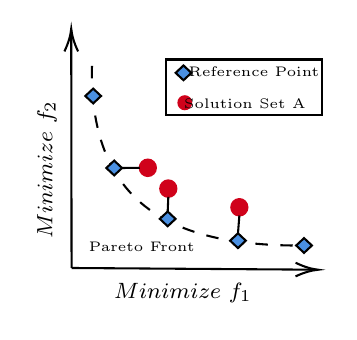
\begin{tikzpicture}[x=0.75pt,y=0.75pt,yscale=-1,xscale=1]
%uncomment if require: \path (0,235); %set diagram left start at 0, and has height of 235

%Straight Lines [id:da6645459220661805] 
\draw    (126.65,152.75) -- (126.49,39.47) ;
\draw [shift={(126.49,37.47)}, rotate = 449.92] [color={rgb, 255:red, 0; green, 0; blue, 0 }  ][line width=0.75]    (10.93,-3.29) .. controls (6.95,-1.4) and (3.31,-0.3) .. (0,0) .. controls (3.31,0.3) and (6.95,1.4) .. (10.93,3.29)   ;

%Straight Lines [id:da25810757520855776] 
\draw    (126.65,152.75) -- (243.5,153.57) ;
\draw [shift={(245.5,153.59)}, rotate = 180.4] [color={rgb, 255:red, 0; green, 0; blue, 0 }  ][line width=0.75]    (10.93,-3.29) .. controls (6.95,-1.4) and (3.31,-0.3) .. (0,0) .. controls (3.31,0.3) and (6.95,1.4) .. (10.93,3.29)   ;

%Curve Lines [id:da9217780493934806] 
\draw  [dash pattern={on 4.5pt off 4.5pt}]  (136.49,55.41) .. controls (134.85,129.62) and (185.36,142.75) .. (241.91,141.91) ;


%Shape: Ellipse [id:dp9288304297821606] 
\draw  [color={rgb, 255:red, 208; green, 2; blue, 27 }  ,draw opacity=1 ][fill={rgb, 255:red, 208; green, 2; blue, 27 }  ,fill opacity=1 ] (159.5,104.47) .. controls (159.5,102.29) and (161.24,100.51) .. (163.39,100.51) .. controls (165.54,100.51) and (167.29,102.29) .. (167.29,104.47) .. controls (167.29,106.66) and (165.54,108.44) .. (163.39,108.44) .. controls (161.24,108.44) and (159.5,106.66) .. (159.5,104.47) -- cycle ;
%Shape: Ellipse [id:dp3466831035198521] 
\draw  [color={rgb, 255:red, 208; green, 2; blue, 27 }  ,draw opacity=1 ][fill={rgb, 255:red, 208; green, 2; blue, 27 }  ,fill opacity=1 ] (203.61,123.51) .. controls (203.61,121.33) and (205.35,119.55) .. (207.5,119.55) .. controls (209.65,119.55) and (211.39,121.33) .. (211.39,123.51) .. controls (211.39,125.7) and (209.65,127.47) .. (207.5,127.47) .. controls (205.35,127.47) and (203.61,125.7) .. (203.61,123.51) -- cycle ;
%Shape: Ellipse [id:dp8431057514843725] 
\draw  [color={rgb, 255:red, 208; green, 2; blue, 27 }  ,draw opacity=1 ][fill={rgb, 255:red, 208; green, 2; blue, 27 }  ,fill opacity=1 ] (169.37,114.51) .. controls (169.37,112.32) and (171.11,110.54) .. (173.27,110.54) .. controls (175.42,110.54) and (177.16,112.32) .. (177.16,114.51) .. controls (177.16,116.69) and (175.42,118.47) .. (173.27,118.47) .. controls (171.11,118.47) and (169.37,116.69) .. (169.37,114.51) -- cycle ;
%Shape: Diamond [id:dp16787571758178776] 
\draw  [color={rgb, 255:red, 0; green, 0; blue, 0 }  ,draw opacity=1 ][fill={rgb, 255:red, 74; green, 144; blue, 226 }  ,fill opacity=1 ] (137.07,66.34) -- (140.86,69.89) -- (137.07,73.45) -- (133.28,69.89) -- cycle ;
%Shape: Diamond [id:dp8884066450256918] 
\draw  [color={rgb, 255:red, 0; green, 0; blue, 0 }  ,draw opacity=1 ][fill={rgb, 255:red, 74; green, 144; blue, 226 }  ,fill opacity=1 ] (147.19,101.02) -- (150.98,104.58) -- (147.19,108.13) -- (143.4,104.58) -- cycle ;
%Shape: Diamond [id:dp7101561956457161] 
\draw  [color={rgb, 255:red, 0; green, 0; blue, 0 }  ,draw opacity=1 ][fill={rgb, 255:red, 74; green, 144; blue, 226 }  ,fill opacity=1 ] (172.96,125.53) -- (176.75,129.09) -- (172.96,132.64) -- (169.17,129.09) -- cycle ;
%Shape: Diamond [id:dp3806535283252863] 
\draw  [color={rgb, 255:red, 0; green, 0; blue, 0 }  ,draw opacity=1 ][fill={rgb, 255:red, 74; green, 144; blue, 226 }  ,fill opacity=1 ] (206.83,136.04) -- (210.62,139.59) -- (206.83,143.15) -- (203.03,139.59) -- cycle ;
%Shape: Diamond [id:dp006261489471205639] 
\draw  [color={rgb, 255:red, 0; green, 0; blue, 0 }  ,draw opacity=1 ][fill={rgb, 255:red, 74; green, 144; blue, 226 }  ,fill opacity=1 ] (238.66,138.36) -- (242.46,141.91) -- (238.66,145.47) -- (234.87,141.91) -- cycle ;
%Straight Lines [id:da45493974031657336] 
\draw    (150.98,104.58) -- (159.5,104.47) ;


%Straight Lines [id:da5268787235096657] 
\draw    (172.96,125.53) -- (173.27,118.47) ;


%Straight Lines [id:da45090976417004924] 
\draw    (207.5,127.47) -- (206.83,136.04) ;


%Shape: Ellipse [id:dp4881097987438625] 
\draw  [color={rgb, 255:red, 208; green, 2; blue, 27 }  ,draw opacity=1 ][fill={rgb, 255:red, 208; green, 2; blue, 27 }  ,fill opacity=1 ] (178.13,73.14) .. controls (178.13,71.41) and (179.5,70.01) .. (181.2,70.01) .. controls (182.9,70.01) and (184.27,71.41) .. (184.27,73.14) .. controls (184.27,74.86) and (182.9,76.26) .. (181.2,76.26) .. controls (179.5,76.26) and (178.13,74.86) .. (178.13,73.14) -- cycle ;
%Shape: Rectangle [id:dp7606725757806145] 
\draw   (171.98,52.31) -- (247.5,52.31) -- (247.5,79) -- (171.98,79) -- cycle ;
%Shape: Diamond [id:dp5520874909126483] 
\draw  [color={rgb, 255:red, 0; green, 0; blue, 0 }  ,draw opacity=1 ][fill={rgb, 255:red, 74; green, 144; blue, 226 }  ,fill opacity=1 ] (180.58,55.18) -- (184.38,58.74) -- (180.58,62.29) -- (176.79,58.74) -- cycle ;

% Text Node
\draw (180.34,164.66) node  [font=\footnotesize]  {$Minimize\ f_{1}$};
% Text Node
\draw (114.77,105.46) node  [font=\footnotesize,rotate=-270.12]  {$Minimize\ f_{2}$};
% Text Node
\draw (160.49,142.48) node  [font=\tiny] [align=left] {Pareto Front};
% Text Node
\draw (210.22,73.49) node  [font=\small] [align=left] {{\tiny Solution Set A}};
% Text Node
\draw (214.5,58.31) node  [font=\small] [align=left] {{\tiny Reference Point}};


\end{tikzpicture}
